\begin{enumerate}[label=\thesection.\arabic*,ref=\thesection.\theenumi]
\item An LC circuit contains a $50 \mu H$ inductor and a $50 \mu F$ capacitor with an initial charge of $10 mC$. The resistance of the circuit is negligible. Let the instant the circuit is closed by $t = 0$.

\textbf{a)} What is the total energy stored initially? Is it conserved during LC oscillations?

\textbf{b)} What is the natural frequency of the circuit?

\textbf{c)} At what time is the energy stored \textbf{(i)} completely electrical (i.e., stored in the capacitor)? \textbf{(ii)} completely magnetic (i.e., stored in the inductor)?

\textbf{d)} At what times is the total energy shared equally between the inductor and the capacitor?

\textbf{e)} If a resistor is inserted in the circuit, how much energy is eventually dissipated as heat? \\
\hfill(NCERT-Physics 12.7 12Q)\\
\solution 
\pagebreak 

\item Obtain the resonant frequency and Q-factor of a series LCR circuit with $L = 3.0\, H$, $C = 27\, \mu F$, and $R = 7.4\, \Omega$. It is desired to improve the sharpness of the resonance of the circuit by reducing its `full width at half maximum' by a factor of 2. Suggest a suitable way.\\
\solution
\iffalse
\let\negmedspace\undefined
\let\negthickspace\undefined
\documentclass[journal,12pt,twocolumn]{IEEEtran}
\usepackage{cite}
\usepackage{amsmath,amssymb,amsfonts,amsthm}
\usepackage{algorithmic}
\usepackage{graphicx}
\usepackage{textcomp}
\usepackage{xcolor}
\usepackage{txfonts}
\usepackage{listings}
\usepackage{enumitem}
\usepackage{mathtools}
\usepackage{gensymb}
\usepackage{comment}
\usepackage[breaklinks=true]{hyperref}
\usepackage{tkz-euclide} 
\usepackage{listings}
\usepackage{gvv}  
\usepackage{tikz}
\usepackage{circuitikz} 
\usepackage{caption}
\def\inputGnumericTable{}              
\usepackage[latin1]{inputenc}          
\usepackage{color}                    
\usepackage{array}                     
\usepackage{longtable}                 
\usepackage{calc}                     \usepackage{multirow}                  
\usepackage{hhline}                    
\usepackage{ifthen}                    
\usepackage{lscape}
\usepackage{amsmath}
\newtheorem{theorem}{Theorem}[section]
\newtheorem{problem}{Problem}
\newtheorem{proposition}{Proposition}[section]
\newtheorem{lemma}{Lemma}[section]
\newtheorem{corollary}[theorem]{Corollary}
\newtheorem{example}{Example}[section]
\newtheorem{definition}[problem]{Definition}
\newcommand{\BEQA}{\begin{eqnarray}}
\newcommand{\EEQA}{\end{eqnarray}}
\newcommand{\define}{\stackrel{\triangle}{=}}
\theoremstyle{remark}
\newtheorem{rem}{Remark}

\begin{document}

\bibliographystyle{IEEEtran}
\vspace{3cm}

\title{NCERT Physics 12.7 Q21}
\author{EE23BTECH11009 - AROSHISH PRADHAN$^{*}$% <-this % stops a space
}
\maketitle
\newpage
\bigskip
\textbf{Question:} 
Obtain the resonant frequency and Q-factor of a series LCR circuit with $L = 3.0\, H$, $C = 27\, \mu F$, and $R = 7.4\, \Omega$. It is desired to improve the sharpness of the resonance of the circuit by reducing its `full width at half maximum' by a factor of 2. Suggest a suitable way.\\

\solution
\fi
Given parameters are:
\begin{table}[!h]
    \centering
    \resizebox{\columnwidth}{!}{
    \begin{tabular}{|c|c|c|}
    \hline
     \textbf{Symbol} & \textbf{Value} &
     \textbf{Description}\\
    \hline
     $L$ &  $3.0\,
     \text{H}$ & Inductance\\
    \hline 
     $C$ &  $27\, \mu\text{F}$ & Capacitance \\
    \hline
     R &  $7.4\, \Omega$ & Resistance\\
    \hline
     Q &  & \parbox{5cm}{Quality Factor: ratio of voltage across inductor or capacitor to that across the resistor at resonance}\\[8pt]
    \hline
     $\omega_0$ & $\dfrac{1}{\sqrt{LC}}$ & Angular Resonant Frequency\\[8pt]
    \hline
\end{tabular}
}
    \vspace{6 pt}
    \caption{Given Parameters}
    \label{tab:1}
\end{table}
\begin{figure}[!h]
 \centering
    \begin{circuitikz}
    \draw(0, 0) -- (1, 0);
    \draw(1, 0) to [L, l = $3.0\text{H}$](2, 0);
    \draw(2, 0) -- (3, 0);
    \draw(3, 0) to [C, l = $27\, \mu\text{F}$](4, 0);
    \draw(4, 0) -- (5, 0);
    \draw(5, 0) to [R, l = $7.4\Omega$](6, 0);
    \draw(0, 0) -- (0, -2);
    \draw[->] (0, -1) node[left] {$I(t)$} -- (0, -1);
    \draw(6, 0) -- (7, 0);
    \draw(7, 0) -- (7, -2);
    \draw(0, -2) -- (3, -2);
    \draw(7, -2) -- (7, -2);
    \draw(3, -2) to [sV, l = $V(t)$](4, -2);
    \draw(4, -2) -- (7, -2);
\end{circuitikz}

    \caption{LCR Circuit}
    \label{fig:enter-label}
\end{figure}
\begin{enumerate}
\item {Frequency Response of the Circuit}

From Kirchhoff's Voltage Law (KVL):
\begin{equation}
V(t) = V_R + V_L + V_C \label{eq:KVL}
\end{equation}
Using reactances from \figref{fig:2},
\begin{align}
    V(s) &= R I(s) + sL I(s) + \dfrac{1}{sC} I(s)\\
    &= I(s)\left(R + Ls + \dfrac{1}{sC}\right)\\
    \implies I(s) &= \dfrac{V(s)}{\left(R + Ls + \dfrac{1}{sC}\right)} \label{eq: 4}
\end{align}
\begin{figure}[!h]
 \centering
    \begin{circuitikz}
    \draw(0, 0) -- (1, 0);
    \draw(1, 0) to [L, l = $sL$](2, 0);
    \draw(2, 0) -- (3, 0);
    \draw(3, 0) to [C, l = $\frac{1}{sC}$](4, 0);
    \draw(4, 0) -- (5, 0);
    \draw(5, 0) to [R, l = $R$](6, 0);
    \draw(0, 0) -- (0, -2);
    \draw[->] (0, -1) node[left] {$I(s)$} -- (0, -1);
    \draw(6, 0) -- (7, 0);
    \draw(7, 0) -- (7, -2);
    \draw(0, -2) -- (3, -2);
    \draw(7, -2) -- (7, -2);
    \draw(3, -2) to [sV, l = $V(s)$](4, -2);
    \draw(4, -2) -- (7, -2);
\end{circuitikz}

    \caption{LCR Circuit}
    \label{fig:2}
\end{figure}
At resonance, the circuit becomes purely resistive. The reactances of capacitor and inductor cancel out as follows:
\begin{align}
    Ls + \dfrac{1}{sC} &= 0\\
    \implies s &= j\dfrac{1}{\sqrt{LC}} \label{eq: 6}
\end{align}
$s$ can be expressed in terms of angular resonance frequency as
\begin{equation}
    s = j\omega_0 \label{eq: 7}
\end{equation}
Comparing \eqref{eq: 6} and \eqref{eq: 7}, we get
\begin{equation}
    \omega_0 = \dfrac{1}{\sqrt{LC}}
\end{equation}
\item{Quality Factor}

\begin{enumerate}
\item Using voltage across inductor,
\begin{align}
    Q &= \left(\dfrac{V_L}{V_R}\right)_{\omega_0} = \dfrac{\lvert{sLI(s)}\rvert}{\lvert RI(s) \rvert}\\
    &= \dfrac{1}{\sqrt{LC}}\dfrac{L}{R}\\
    &= \dfrac{1}{R}\sqrt{\dfrac{L}{C}}
\end{align}
\item Using voltage across capacitor,
\begin{align}
	Q &= \left(\dfrac{V_C}{V_R}\right)_{\omega_0} = \dfrac{\abs{\frac{I(s)}{sC}}}{\lvert RI(s) \rvert}\\
    &= \dfrac{\sqrt{LC}}{RC}\\
    &= \dfrac{1}{R}\sqrt{\dfrac{L}{C}}
\end{align}
\end{enumerate}
\item{Plot of Impedance vs Angular Frequency}

Impedance is defined as
\begin{equation}
    H(s) = \dfrac{V(s)}{I(s)}
\end{equation}
Using \eqref{eq: 4},
\begin{align}
     H(s) &= R + sL + \dfrac{1}{sC}\\
     \implies H(j\omega) &= R + j\omega L + \dfrac{1}{j\omega C}\\
     \implies \lvert H(j\omega) \rvert &= \sqrt{R^2 + \left(\omega L - \dfrac{1}{\omega C}\right)^2}
\end{align}
\begin{figure}[!h]
    \centering
    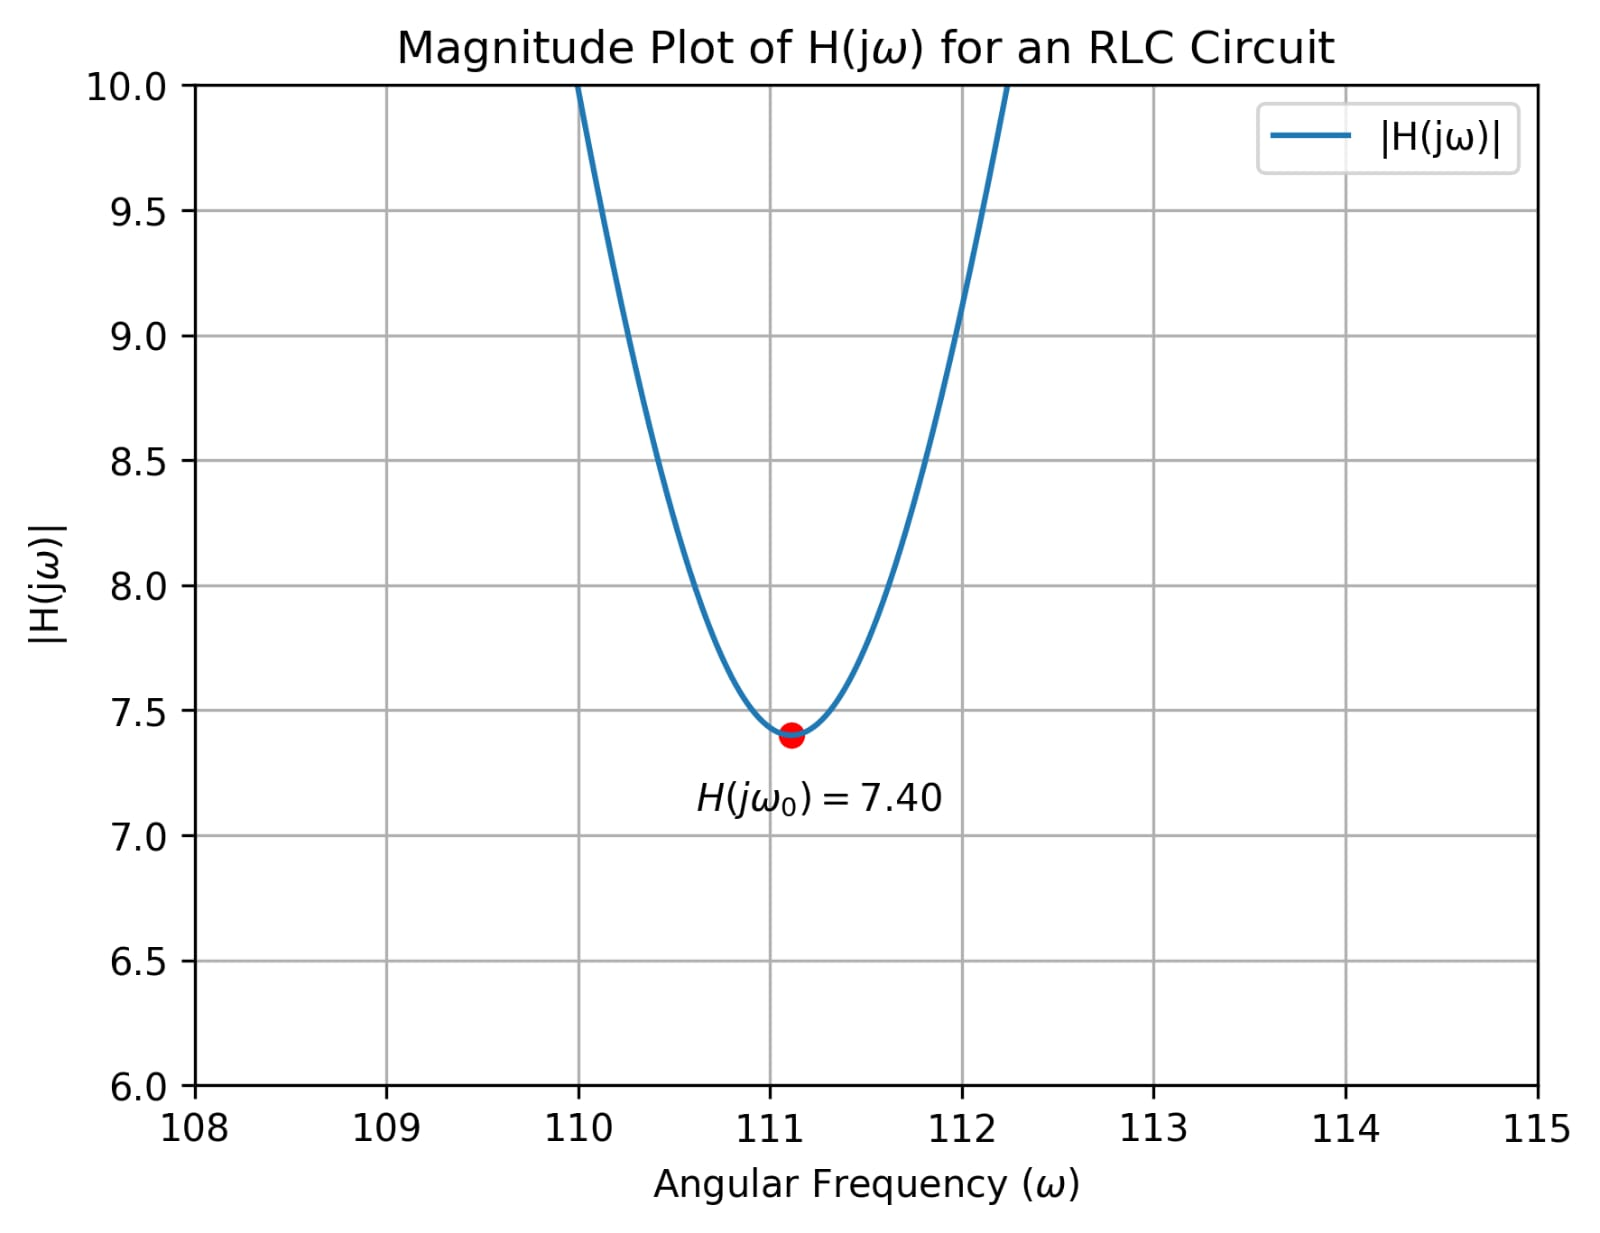
\includegraphics[width = \columnwidth]{ncert-physics/12/7/21/h_plot.png}
    \caption{Impedance vs $\omega$ (using values in \tabref{tab:1})}
    \label{fig:h_plot}
\end{figure}
\end{enumerate}


\pagebreak
\item A circuit containing a $80 mH$ inductor and a $60 \mu F$ capacitor in series is connected to a $230 V$, $50 Hz$ supply. A resistance of $15 \Omega $ is connected in series. Obtain the average power transferred to each element of the circuit, and the total power absorbed.\\
\solution
\pagebreak

\item A series LCR circuit with 
\(L = 0.12 \, \text{H}\),
\(C = 480 \times 10^{-9} \, \text{F}\), 
\(R=23 \, \Omega\)
is connected to a 230 V variable frequency supply.
(a) What is the source frequency for which current amplitude is maximum? Obtain this maximum value.

(b) What is the source frequency for which the average power absorbed by the circuit is maximum? Obtain the value of this maximum power.

(c) For which frequencies of the source is the power transferred to the circuit half the power at resonant frequency? What is the current amplitude at these frequencies?

(d) What is the Q-factor of the given circuit?
\end{enumerate}
